%----------------------------------------------------------------------------
%
%	This template was created by
%		Christian Krieg <christian.krieg@alumni.tuwien.ac.at>
%
%	April 2018
%
%----------------------------------------------------------------------------
%
\documentclass[%
	a4paper,
]
{article}
%
%----------------------------------------------------------------------------
%
% Institution
%
%\institution{Institute of Computer Technology}
%
%----------------------------------------------------------------------------
%
% Use the 'Libertine' font type
%
\usepackage{libertine}
\usepackage[T1]{fontenc}
\usepackage[utf8]{inputenc}
%
%----------------------------------------------------------------------------
%
% Set page margins
%
\usepackage{geometry}
\geometry{%
	left   = 2cm,
	right  = 2cm,
	top    = 2cm,
	bottom = 2cm
}
%
%----------------------------------------------------------------------------
%
% Set line spacing
%
\usepackage{setspace}
\setstretch{1}
%
%----------------------------------------------------------------------------
%
% Set paragraph: No indentation, but include an empty line
%
\usepackage[parfill]{parskip}
%
%----------------------------------------------------------------------------
%
% Settings for hyperlinks
%
\usepackage{hyperref}
\hypersetup{%
	colorlinks = true,
	allcolors  = blue,
}
%
%----------------------------------------------------------------------------
%
% Use colors
%
\usepackage{xcolor}
\usepackage{colortbl}
%
%----------------------------------------------------------------------------
%
% Define a TODO and a DONE command
%
\newcommand{\todo}[1]{\textcolor{red}{#1}}
\newcommand{\done}[1]{}
%
%----------------------------------------------------------------------------
%
% Use glossaries
%
\usepackage{glossaries}
\makeglossaries
%
% Glossary entries
%
\newglossaryentry{fpga}{
	name = {FPGA},
	description = {Field-programmable gate array},
	text = {FPGA},
	first = {field-programmable gate array (FPGA)},
	plural = {FPGAs},
	firstplural = {field-programmable gate arrays (FPGAs)},
}
%
\newglossaryentry{trng}{
	name = {TRNG},
	description = {True-random number generator},
	text = {TRNG},
	first = {true-random number generator (TRNG)},
	plural = {TRNGs},
	firstplural = {true-random number generators (TRNGs)},
}
%
\newglossaryentry{bcd}{
  name={BCD},
  description={Binary-coded decimal},
  text={BCD},
  first={binary-coded decimal (BCD)},
}
%
\newglossaryentry{hdl}{
  name={HDL},
  description={Hardware description language},
  text={HDL},
  first={hardware description language (HDL)},
  plural={HDLs},
  firstplural={hardware description languages (HDLs)},
}
%
\newglossaryentry{ip}{
  name={IP},
  description={Intellectual property},
  text={IP},
  first={intellectual property (IP)},
}
%
\newglossaryentry{3pip}{
  name={3PIP},
  description={Third-party intellectual property},
  text={3PIP},
  first={third-party intellectual property (3PIP)},
}
%
\newglossaryentry{dsp}{
  name={DSP},
  description={Digital signal processor},
  text={DSP},
  first={digital signal processor (DSP)},
  plural={DSPs},
  firstplural={digital signal processors (DSPs)},
}
%
\newglossaryentry{amba}{
  name={AMBA},
  description={Advanced microcontroller bus architecture},
  text={AMBA},
  first={advanced microcontroller bus architecture (AMBA)},
}
%
\newglossaryentry{apb}{
  name={APB},
  description={Advanced peripheral bus},
  text={APB},
  first={advanced peripheral bus (APB)},
}
%
%\newglossaryentry{}{
%  name={},
%  description={},
%  text={},
%  first={},
%  plural={},
%  firstplural={},
%}
%
%----------------------------------------------------------------------------
%
% Using URLs
%
\usepackage{url}
%
%
%% Define a new style with a smaller font.
\makeatletter
\def\url@footnotestyle{%
  \@ifundefined{selectfont}{\def\UrlFont{\sf}}{\def\UrlFont{\footnotesize\rmfamily}}}
\makeatother
%% Now actually use the newly defined style.
\urlstyle{footnote}
%
%
%
%% Define a new style with a larger font.
\makeatletter
\def\url@normalstyle{%
  \@ifundefined{selectfont}{\def\UrlFont{\sf}}{\def\UrlFont{\normalsize\rmfamily}}}
\makeatother
%% Now actually use the newly defined style.
\urlstyle{footnote}
%
%----------------------------------------------------------------------------
%
% Settings for citations and the bibliography
%
\usepackage[%
	backend     = biber,
	maxbibnames = 99,
	autocite    = footnote,
	citestyle   = verbose-ibid,
	firstinits=true,
]{biblatex}
\bibliography{bib/task-2}
%
%----------------------------------------------------------------------------
%
%	TikZ -- TikZ ist kein Zeichenprogramm
%
\usepackage{tikz}
\usepackage{tikz-timing}
\usepackage{etoolbox}
\usetikzlibrary{mindmap}
\usetikzlibrary{shapes}
\usetikzlibrary{arrows}
\usetikzlibrary{decorations}
\usetikzlibrary{shapes.symbols}
\usetikzlibrary{shapes.geometric}
\usetikzlibrary{shapes.multipart}
\usetikzlibrary{positioning}
\usetikzlibrary{patterns}
\usetikzlibrary{calc}
\usetikzlibrary{scopes}         % cf. pgfmanual p.66
\usetikzlibrary{chains}         % cf. pgfmanual p.284
\usetikzlibrary{fit}
\usetikzlibrary{matrix}
\usetikzlibrary{decorations}
\usetikzlibrary{circuits.logic}
\usetikzlibrary{circuits.logic.IEC}
\usetikzlibrary{shapes.gates.logic.IEC}
\usetikzlibrary{circuits.logic.US}
\usetikzlibrary{shapes.gates.logic.US}
\usetikzlibrary{circuits.ee}
\usetikzlibrary{circuits.ee.IEC}
\usetikzlibrary{backgrounds}
\usetikzlibrary{automata}
\usetikzlibrary{intersections}
\usetikzlibrary{plotmarks}
\usepgflibrary{fpu}
\usetikzlibrary{decorations.pathreplacing}
%
%----------------------------------------------------------------------------
%
% TikZ shapes
%  
%	% D flip-flops (DFFs) and shift register
% Author: Martin Scharrer
%\documentclass[a4paper,landscape]{article}

%\usepackage{pgf,tikz}
%%%<
%\usepackage{verbatim}
%\usepackage[active,tightpage]{preview}
%\PreviewEnvironment{tikzpicture}
%\setlength\PreviewBorder{5pt}%
%%%>

%\begin{comment}
%:Title: D flip-flops and shift register
%
%Example of a custom node shape for drawing  D flip-flops. The shape is used to draw a serial shift
%register. 
%
%\end{comment}
%
%\usetikzlibrary{calc,arrows}
%\usepackage{amsmath}
%\usepackage[left=1cm,right=1cm]{geometry}
%\pagestyle{empty}

\makeatletter

% Data Flip Flip (DFF) shape
\pgfdeclareshape{dff}{
  % The 'minimum width' and 'minimum height' keys, not the content, determine
  % the size
  \savedanchor\northeast{%
    \pgfmathsetlength\pgf@x{\pgfshapeminwidth}%
    \pgfmathsetlength\pgf@y{\pgfshapeminheight}%
    \pgf@x=0.5\pgf@x
    \pgf@y=0.5\pgf@y
  }
  % This is redundant, but makes some things easier:
  \savedanchor\southwest{%
    \pgfmathsetlength\pgf@x{\pgfshapeminwidth}%
    \pgfmathsetlength\pgf@y{\pgfshapeminheight}%
    \pgf@x=-0.5\pgf@x
    \pgf@y=-0.5\pgf@y
  }
  % Inherit from rectangle
  \inheritanchorborder[from=rectangle]

  % Define same anchor a normal rectangle has
  \anchor{center}{\pgfpointorigin}
  \anchor{north}{\northeast \pgf@x=0pt}
  \anchor{east}{\northeast \pgf@y=0pt}
  \anchor{south}{\southwest \pgf@x=0pt}
  \anchor{west}{\southwest \pgf@y=0pt}
  \anchor{north east}{\northeast}
  \anchor{north west}{\northeast \pgf@x=-\pgf@x}
  \anchor{south west}{\southwest}
  \anchor{south east}{\southwest \pgf@x=-\pgf@x}
  \anchor{text}{
    \pgfpointorigin
    \advance\pgf@x by -.5\wd\pgfnodeparttextbox%
    \advance\pgf@y by -.5\ht\pgfnodeparttextbox%
    \advance\pgf@y by +.5\dp\pgfnodeparttextbox%
  }

  % Define anchors for signal ports
  \anchor{D}{
    \pgf@process{\northeast}%
    \pgf@x=-1\pgf@x%
    \pgf@y=.5\pgf@y%
  }
  \anchor{CLK}{
    \pgf@process{\northeast}%
    \pgf@x=-1\pgf@x%
    \pgf@y=-.66666\pgf@y%
  }
  \anchor{CE}{
    \pgf@process{\northeast}%
    \pgf@x=-1\pgf@x%
    \pgf@y=-0.33333\pgf@y%
  }
  \anchor{Q}{
    \pgf@process{\northeast}%
    \pgf@y=.5\pgf@y%
  }
  \anchor{Qn}{
    \pgf@process{\northeast}%
    \pgf@y=-.5\pgf@y%
  }
  \anchor{R}{
    \pgf@process{\northeast}%
    \pgf@x=0pt%
  }
  \anchor{S}{
    \pgf@process{\northeast}%
    \pgf@x=0pt%
    \pgf@y=-\pgf@y%
  }
  % Draw the rectangle box and the port labels
  \backgroundpath{
    % Rectangle box
    \pgfpathrectanglecorners{\southwest}{\northeast}
    % Angle (>) for clock input
    \pgf@anchor@dff@CLK
    \pgf@xa=\pgf@x \pgf@ya=\pgf@y
    \pgf@xb=\pgf@x \pgf@yb=\pgf@y
    \pgf@xc=\pgf@x \pgf@yc=\pgf@y
    \pgfmathsetlength\pgf@x{.75ex} % size depends on font size
    \advance\pgf@ya by \pgf@x
    \advance\pgf@xb by \pgf@x
    \advance\pgf@yc by -\pgf@x
    \pgfpathmoveto{\pgfpoint{\pgf@xa}{\pgf@ya}}
    \pgfpathlineto{\pgfpoint{\pgf@xb}{\pgf@yb}}
    \pgfpathlineto{\pgfpoint{\pgf@xc}{\pgf@yc}}
    \pgfclosepath

    % Draw port labels
    \begingroup
    \tikzset{flip flop/port labels} % Use font from this style
    \tikz@textfont

    \pgf@anchor@dff@D
    \pgftext[left,base,at={\pgfpoint{\pgf@x}{\pgf@y}},x=\pgfshapeinnerxsep]{\raisebox{-0.75ex}{D}}

%    \pgf@anchor@dff@CE
%    \pgftext[left,base,at={\pgfpoint{\pgf@x}{\pgf@y}},x=\pgfshapeinnerxsep]{\raisebox{-0.75ex}{CE}}

    \pgf@anchor@dff@Q
    \pgftext[right,base,at={\pgfpoint{\pgf@x}{\pgf@y}},x=-\pgfshapeinnerxsep]{\raisebox{-.75ex}{Q}}

%    \pgf@anchor@dff@Qn
%    \pgftext[right,base,at={\pgfpoint{\pgf@x}{\pgf@y}},x=-\pgfshapeinnerxsep]{\raisebox{-.75ex}{$\overline{\mbox{Q}}$}}
%
%    \pgf@anchor@dff@R
%    \pgftext[top,at={\pgfpoint{\pgf@x}{\pgf@y}},y=-\pgfshapeinnerysep]{R}
%
%    \pgf@anchor@dff@S
%    \pgftext[bottom,at={\pgfpoint{\pgf@x}{\pgf@y}},y=\pgfshapeinnerysep]{S}
    \endgroup
  }
}

% Key to add font macros to the current font
\tikzset{add font/.code={\expandafter\def\expandafter\tikz@textfont\expandafter{\tikz@textfont#1}}} 

% Define default style for this node
% \tikzset{flip flop/port labels/.style={font=\sffamily\scriptsize}}
%\tikzset{every dff node/.style={draw,minimum width=2cm,minimum 
%height=2.828427125cm,very thick,inner sep=1mm,outer sep=0pt,cap=round,add 
%font=\sffamily}}
\tikzset{flip flop/port labels/.style={font=\tiny}}
\tikzset{every dff node/.style={draw,minimum width=.75cm,minimum 
height=1cm,inner sep=1mm,outer sep=0pt,cap=round,font=\scriptsize}}

\makeatother

%\begin{document}
%
%\begin{tikzpicture}[font=\sffamily,>=triangle 45]
%  \def\N{7}  % Number of Flip-Flops minus one
%
%  % Place FFs
%  \foreach \m in {0,...,\N}
%    \node [shape=dff] (DFF\m) at ($ 3*(\m,0) $) {Bit \#\m};
%
%  % Connect FFs (Q1 with D1, etc.)
%  \def\p{0}  % Used to save the previous number
%  \foreach \m in {1,...,\N} { % Note that it starts with 1, not 0
%    \draw [->] (DFF\p.Q) -- (DFF\m.D);
%    \global\let\p\m
%  }
%
%  % Connect and label data in- and output port
%  \draw [<-] (DFF0.D) -- +(-1,0) node [anchor=east] {input} ;
%  \draw [->] (DFF\N.Q) -- +(1,0) node [anchor=west] {output};
%
%  % 'Reset' port label
%  \path (DFF0) +(-2cm,+2cm) coordinate (temp)
%    node [anchor=east] {reset};
%  % Connect resets
%  \foreach \m in {0,...,\N}
%    \draw [->] (temp) -| (DFF\m.R);
%
%  % 'Set' port label
%  \path (DFF0) +(-2cm,-2cm) coordinate (temp)
%    node [anchor=east] {set};
%  % Connect sets
%  \foreach \m in {0,...,\N}
%    \draw [->] (temp) -| (DFF\m.S);
%
%  % Clock port label
%  \path (DFF0) +(-2cm,-2.5cm) coordinate (temp)
%    node [anchor=east] {clock};
%  \foreach \m in {0,...,\N}
%    \draw [->] (temp) -| ($ (DFF\m.CLK) + (-5mm,0) $) --(DFF\m.CLK);
%
%  % Clock port label
%  \path (DFF0) +(-2cm,-3cm) coordinate (temp)
%    node [anchor=east] {clock enable};
%  \foreach \m in {0,...,\N}
%    \draw [->] (temp) -| ($ (DFF\m.CE) + (-7.5mm,0) $) --(DFF\m.CE);
%\end{tikzpicture}
%
%\end{document}

%
%----------------------------------------------------------------------------
%
% Use AMS math fonts
%
\usepackage{amsfonts}
\usepackage[sans]{dsfont}
%
%----------------------------------------------------------------------------
%
% Use multiple figures in one float
%
\usepackage{subcaption}
%
%----------------------------------------------------------------------------
%
% Use dummy text
%
\usepackage{lipsum}
%
%----------------------------------------------------------------------------
%
% Use extended list environments (e.g., 'inparaenum')
%
\usepackage{paralist}
%
%----------------------------------------------------------------------------
%
% Use listings
%
\usepackage{listings}

\lstdefinestyle{vhdl}
{
	language=VHDL,
  basicstyle=\linespread{1}\scriptsize\ttfamily\color{black},
  commentstyle=\scriptsize\itshape,
  escapeinside={(*@}{@*)},
  frame=single, numbers=left,
%  numbersep=5pt,
  xleftmargin=15pt,
  xrightmargin=5pt,
  numbersep=5pt,
  breaklines=true,
  moredelim=**[is][\ttfamily\bfseries\color{red}]{(*}{*)},
}

\lstdefinestyle{verilog}
{
	language=Verilog,
  basicstyle=\linespread{1}\scriptsize\ttfamily\color{black},
  commentstyle=\scriptsize\itshape,
  escapeinside={(*@}{@*)},
  frame=single, numbers=left,
%  numbersep=5pt,
  xleftmargin=15pt,
  xrightmargin=5pt,
  numbersep=5pt,
  breaklines=true,
  moredelim=**[is][\ttfamily\bfseries\color{red}]{(*}{*)},
}
%
%----------------------------------------------------------------------------
%
% Typeset pseudo code
%
\usepackage{syntax}
%
%----------------------------------------------------------------------------
%
% More options for boxes
%
\usepackage{realboxes}
%
% Command for vertical text in tabulars
%
\newcommand*\rot{\rotatebox{90}}
%
%----------------------------------------------------------------------------
%
% Use \textsubscript
%
\usepackage{fixltx2e}
%
%----------------------------------------------------------------------------
%
% More options for tabulars
%
\usepackage{array}
%
%----------------------------------------------------------------------------
%
% Use appendices
%
\usepackage[titletoc]{appendix}
%
%----------------------------------------------------------------------------
%
% Use the cleverref package -- Load this package as the very last!
%
\usepackage{cleveref}


\usepackage{import}
\usepackage{xifthen}
\usepackage{pdfpages}
\usepackage{transparent}

\newcommand{\incfig}[2]{%
    \def\svgscale{#2}
    \import{./fig/}{#1.pdf_tex}
}


\newcommand{\DrawData}[5]{
        \draw plot [mark=#1, mark size=50,  mark options={#2}] coordinates{( #3 , #4 , #5 )}; 
        \draw[very thin,gray] ( #3 , 0 , #5 ) -- ( #3 , #4 , #5 ) node[right] { (#3 #4 #5)} ;
        \draw[very thin,gray] ( #3 , 0 , #5 ) -- ( #3 , 0 , 0 ) ;
        \draw[very thin,gray] ( #3 , 0 , #5 ) -- ( 0 , 0 , #5 ) ;
}
\newcommand{\DrawDataUnmarked}[5]{
        \draw plot [mark=#1, mark size=50,  mark options={#2}] coordinates{( #3 , #4 , #5 )}; 
        \draw[very thin,gray] ( #3 , 0 , #5 ) -- ( #3 , #4 , #5 ) ;
        \draw[very thin,gray] ( #3 , 0 , #5 ) -- ( #3 , 0 , 0 ) ;
        \draw[very thin,gray] ( #3 , 0 , #5 ) -- ( 0 , 0 , #5 ) ;
}

\usepackage{float}
\usepackage{graphicx}
\usepackage{rotating}
\usepackage{pdflscape}
%
%----------------------------------------------------------------------------
%
% Document body
%
\begin{document}
%
%----------------------------------------------------------------------------
%
\begin{titlepage}

	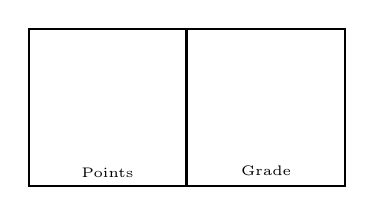
\begin{tikzpicture}[thick]
		\node (points) at (0,0) [draw,minimum size=2cm] {};
		\node (lbl-points) at (points.south) [anchor=south,font=\tiny] {Points};
		\node (grade) at (points.east) [draw,minimum size=2cm,anchor=west,
			outer sep=0] {};
		\node (lbl-grade) at (grade.south) [anchor=south,font=\tiny] {Grade};
	\end{tikzpicture}

	\begin{flushright}

		% Update this with your team number
		\huge\bfseries
		Team: XX \\[1em]

		% Update this with your matriculation number, first name, second name
		\large
		MatNr. First SECOND \#1	\\
		MatNr. First SECOND \#2	\\
		... \\
	
	\end{flushright}

	\vspace{5em}

	\begin{center}
		{\huge Digital Integrated Circuits Lab (LDIS)}\\[1em]
		{\Large 384.088, Summer Term 2019} \\[2em]
		{\large Supervisors:\\[.5em]
			Christian Krieg, David Radakovits, Axel Jantsch} \\[10em]

		{\Huge Task 2:\\[.5em]Design Characterization,\\[.5em]Bus Communication}\\[10em]
	\end{center}


%	\begin{abstract}
%
%		Enter the abstract of your report here. An abstract summarizes your
%		entire work (i.e., problem statement, motivation, methodology, key
%		findings). It is a good strategy to write a first version of the abstract
%		when you start to work on your report. This gives you a good guideline
%		what to	put and what not to put into the report. Ideally, you re-write
%		the abstract once you finished your report, because only at this point
%		you have all the information available to create a good abstract.
%
%	\end{abstract}

\end{titlepage}
%
%----------------------------------------------------------------------------
%
\section{Characterize your design from Task 1}
\label{sec:characterization}

In order to make your design implementation comparable to other
implementations, simulate your design using Vivado and perform the
following measurements:

\begin{enumerate}

	\item{Timing analysis}

	\item{Power analysis}

	\item{Resource consumption}

\end{enumerate}

Create a design space vector for your design.%
The design space vector holds the following parameters, where $t_{max}$
is the maximum delay for the critical path, $P_{avg}$ is the average
power consumption for your design (vector-less post-place-and-route power
estimation), and $r$ is the percentage of resources used in your
implementation for the Nexys 4 DDR board (for sake of simplicity, use the
percentage of slices):

\begin{align}
	\vec{v} =
		\begin{bmatrix}
		t_{max}  \\
		P_{avg}\\
		r  \\
	\end{bmatrix}
\end{align}

You will find information on power estimation~\autocite{xpe} and timing
analysis~\autocite{timing} on the web.

Get the design space vectors of your colleagues, and visualize the
three-dimensional design space. Use black crosses for the vectors of your
colleagues, and a filled circle for your own vector.
%
%----------------------------------------------------------------------------
%
\section{Create an AMBA APB interface}

The goal of this subtask is to make your design accessible from other
\gls{ip} cores via the \gls{amba} \gls{apb}. Consult the \gls{apb}
specification~\autocite{apb}, and:

\begin{enumerate}

	\item{Implement a bus controller that implements the use case for your
		task}

	\item{Implement a bus interface for any sub-component of your design
		from Task~1 (sampling, data processing, output).}

	\item{Implement a module that takes the user input for runtime parameters
		and connect it to the bus}

\end{enumerate}

\begin{figure}[h!]
	\centering
	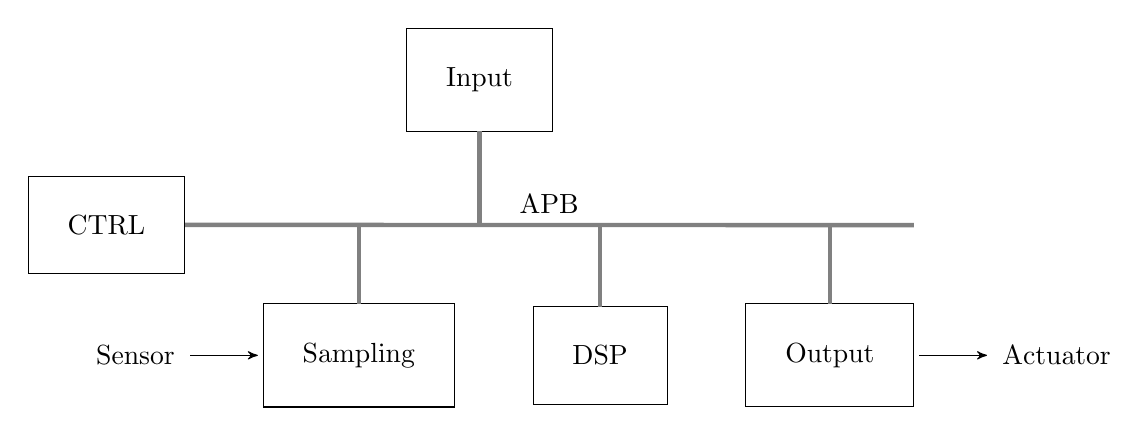
\begin{tikzpicture}[
	nd/.append style={draw, minimum height=1cm, inner sep=5mm, outer sep=0, align=center},
	ed/.style={->, >= stealth', shorten >=2pt, shorten <= 2pt},
]

	\node(input)[nd]{Sampling};
	\node(dsp)[nd, right=of input]{DSP};
	\node(output)[nd, right=of dsp]{Output};
	\node(userinput) at ($ (input)!.5!(dsp) +(0,3.5) $) [nd] {Input};

	\draw[ed,<-] (input.west) -- ++(-1cm,0) node[left]{Sensor};
%	\draw[ed] (input) -- (dsp);
%	\draw[ed] (dsp) -- (output);
	\draw[ed] (output.east) -- ++(1cm,0) node[right]{Actuator};

	\begin{scope}[ultra thick, gray]
		\draw ($ (input.north west) + (-1cm,1cm) $) coordinate(bus) -- node [above,midway,black] {APB} ($ (output.north east) +(0,1cm) $);
		\draw (input) -- (input |- bus);
		\draw (dsp) -- (dsp |- bus);
		\draw (output) -- (output |- bus);
		\draw (userinput) -- (userinput |- bus);
	\end{scope}

	\node (ctrl) at (bus) [nd,anchor=east]{CTRL};

\end{tikzpicture}
	\caption{System of Task~1 equipped with an \gls{apb}}
	\label{fig:audio-block}
\end{figure}

Your system should be able to take the user input, parametrize the system
according to the user input, and perform the actual task. Instead of
directly connecting each of the sub-components directly, the modules should
communicate over the \gls{apb}. The audio system can be treated as one
module; as it is kind of a real-time system, it wouldn't make a lot of sense
to let it communicate over the \gls{apb}. The user-input (e.g., cut-off
freuqency) should be set over the \gls{apb}.
%
%----------------------------------------------------------------------------
%
\section{Characterization}
\begin{table}[ht]
    \centering
    \begin{tabular}{l|lll}
         Group & $\text{t}_\text{{max}} [\text{ns}]	$ & $\text{P}_\text{avg} [\text{mW}]$ & $\text{r} [\%] $ \\ \hline \hline
        Philipp, Benedikt &	5,44	& 88,00	& 6,60 \\
        Kratzmann &	5,03 &	185,00 & 13,12 \\
        Essbüchl Jakob &	37,62 &	140	& 1,36 \\
        Glinserer Andreas &	5,89 &	110	& 1,54 \\ 
        Hauk Raphael &	8,08 &	111 &	3,9 \\
        Philipp W. &	2,557 &	121 &	0,477\\
        \hline
    \end{tabular}
    \caption{table with the values}
    \label{tab:my_label}
\end{table}

\begin{figure}[H]
    \centering
    \resizebox{.4\textwidth}{!}{
        \begin{tikzpicture}[scale=0.04,x = {(0.866cm,0.5cm)}, y={(0cm,1cm)}, z={(0.866cm,-0.5cm)},]
            \draw[thin,->] (0,0,0)     -- (40,0,0) node[right] {$t_{max}$}   node[above left]    {40};
            \draw[thin,->] (0,0,0)     -- (0,220,0) node[above] {$P_{avg}$}   node[left]          {220};
            \draw[thin,->] (0,0,0)     -- (0,0,15) node[right] {$r$}           node[below left]    {15};
            \DrawDataUnmarked{o}{black}{5.89}{110}{1.54} % mine
            % others
            \DrawData{x}{red}{5.44} {88}    {6.6}
            \DrawData{x}{red}{5.03} {185}   {13.12}
            \DrawData{x}{red}{37.62}{140}   {1.36} 
            \DrawData{x}{red}{8.08} {111}   {3.9}
            \DrawData{x}{red}{2.557}{121}   {0.477}

        \end{tikzpicture}
    }
    \caption{visualization of table}
    \label{fig:my_label}
\end{figure}

\section{Implementation}

My implementation is as follows: I have additional registers in front of every
instantiated component. The APB bus then reads and writes into/from these 
registers. Due the lack of documentation I implemented the PREADY signal with
a tristates. It would also be possible to implement this as a wire for each
module on its own.

\subsection{Master CTRL}
The master is amplemented with 2 state machines. 
Every state machine is implemented with 2 processes. 1 process
which handles the outputs and another process which handles
the evaluation of the next state. The state change happens in
a synchronous process.
1 of the state
machines handles the APB Protocol and Data exchange on the line. 
It is built after the state machine (fig.\ref{fig:apb-state}) in the AMBA protocol pdf.

\begin{figure}[ht]
    \centering
    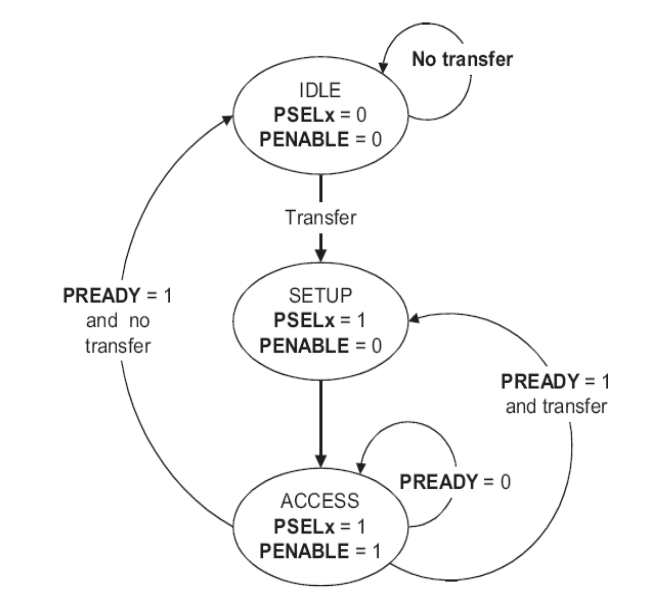
\includegraphics[scale=0.3]{fig/apb-state-diag.png}
    \caption{APB state diagram. Source:\protect\autocite{apb}}
    \label{fig:apb-state}
\end{figure}

The second state machine handles the program procedure (fig.\ref{fig:mst-state}). The 
procedure is as follows: Every $100\,\text{ms}$ it checks if
the switches changed. If a change happened then the new size
gets transmitted to the DSP. Every 
$\dfrac{1}{\text{samples}}\,\text{s}$ it reads the
Sampling part, writes this data then to the DSP, reads the DSP
and then transmits the output from the DSP to the output.

\begin{figure}[ht]
    \centering
    \incfig{master-state-diagram}{1.7}
    \caption{master state diagram. Source: Drawn in Inkscape}
    \label{fig:mst-state}
\end{figure}


\subsection{APB slaves}
The slaves were implemented with the goal to leave the working
parts untouched. This goal was reached by implementing the
slaves as registers. The master writes to the registers and
the slave component reads from the register. Therefore every
slave looks the same with slight modifications:

\lstset{style=vhdl}
\begin{lstlisting}
enable_write <= in_PENABLE and in_PWRITE and in_PSELx;
enable_read  <= not in_PWRITE and in_PSELx;     -- data is read everytime to be ready on the first cycle

out_PREADY <= int_pready;

-- register with the enable sigs as clock
WRITE: process(in_PRESETn, enable_write)
begin
        if in_PRESETn ='1' then
                int_data_write <= x"0000";

        elsif rising_edge(enable_write) then
                int_data_write <= in_PWDATA;
        end if;
end process WRITE;

-- register with the enable sigs as clock
READ: process(in_PRESETn, enable_read)
begin
        if in_PRESETn ='1' then
                out_PRDATA <= x"0000";

        elsif rising_edge(enable_read) then
                out_PRDATA <= int_data_read;

        end if;
end process WRITE;

PREADYP: process(enable_write, enable_read)
begin
        if enable_write='1' or enable_read='1' then
                int_PREADY <= '1';
        else
                int_PREADY <= '0';
        end if;
end process PREADYP;

-- process to forward the data to whatever module or to write into the read register
SFORWARD: process(in_PRESETn, in_PCLK, enable_write, in_PADDR)
begin

        if rising_edge(in_PCLK) then
                if in_PRESETn = '0' then
                        int_data_read <= x"0000";
                else
                        -- here comes handling of signals to write into the read register

                end if; -- rst
        end if; -- rising clock
end process SFORWARD;
\end{lstlisting}

For every slave a new .vhd file was created with the template above in it and an 
instantiation of the component it is the interface to. The ADT slave samples values
and if the CTRL requests values faster it just gets the old value back. If you write
to the DSP part, the DSP holds the bus transmission by holding the PREADY signal low
until the new value is computed.

\subsection{LEDs}
\begin{table}[ht]
    \centering
    \begin{tabular}{|l|l|l|l|l|l|l|l|}
        \hline
         LD15 & LD14 & LD13 & LD12 & LD11 & LD10 & LD09 & LD08 \\ \hline
         \multicolumn{8}{|c|}{Buffer size of the DSP binary encoded} \\ \hline
         \multicolumn{8}{c}{} \\ \hline
         LD07 & LD06 & LD05 & LD04 & LD03 & LD02 & LD01 & LD00 \\ \hline
         ADT & \multicolumn{3}{c|}{CTRL size} & STATE & \multicolumn{3}{c|}{DSP size} \\ \hline
    \end{tabular}
    \caption{LED explanation}
    \label{tab:leds}
\end{table}

\begin{itemize}
    \item ADT - signals everytime the ADT samples a new value
    \item CTRL size - the size saved in CTRL part as power of two. 
        E.g. $\text{b'}1 1 0 = 6 -> 2^6 = 64$ buffer size.
    \item STATE - toggles everytime the CTRL goes into the idle state
    \item DSP size - same as CTRL size but saved in the DSP part
\end{itemize}

\subsection{Simulation}
Here are two images from the simultion. The first one shows the way
the master works in respect to polling the switch slave. The switch
slave select wire is choosen more often. And corresponding to the 
countersize it starts a normal cycle. The normal cycle can be seen in 
the second simulation image.
\newpage

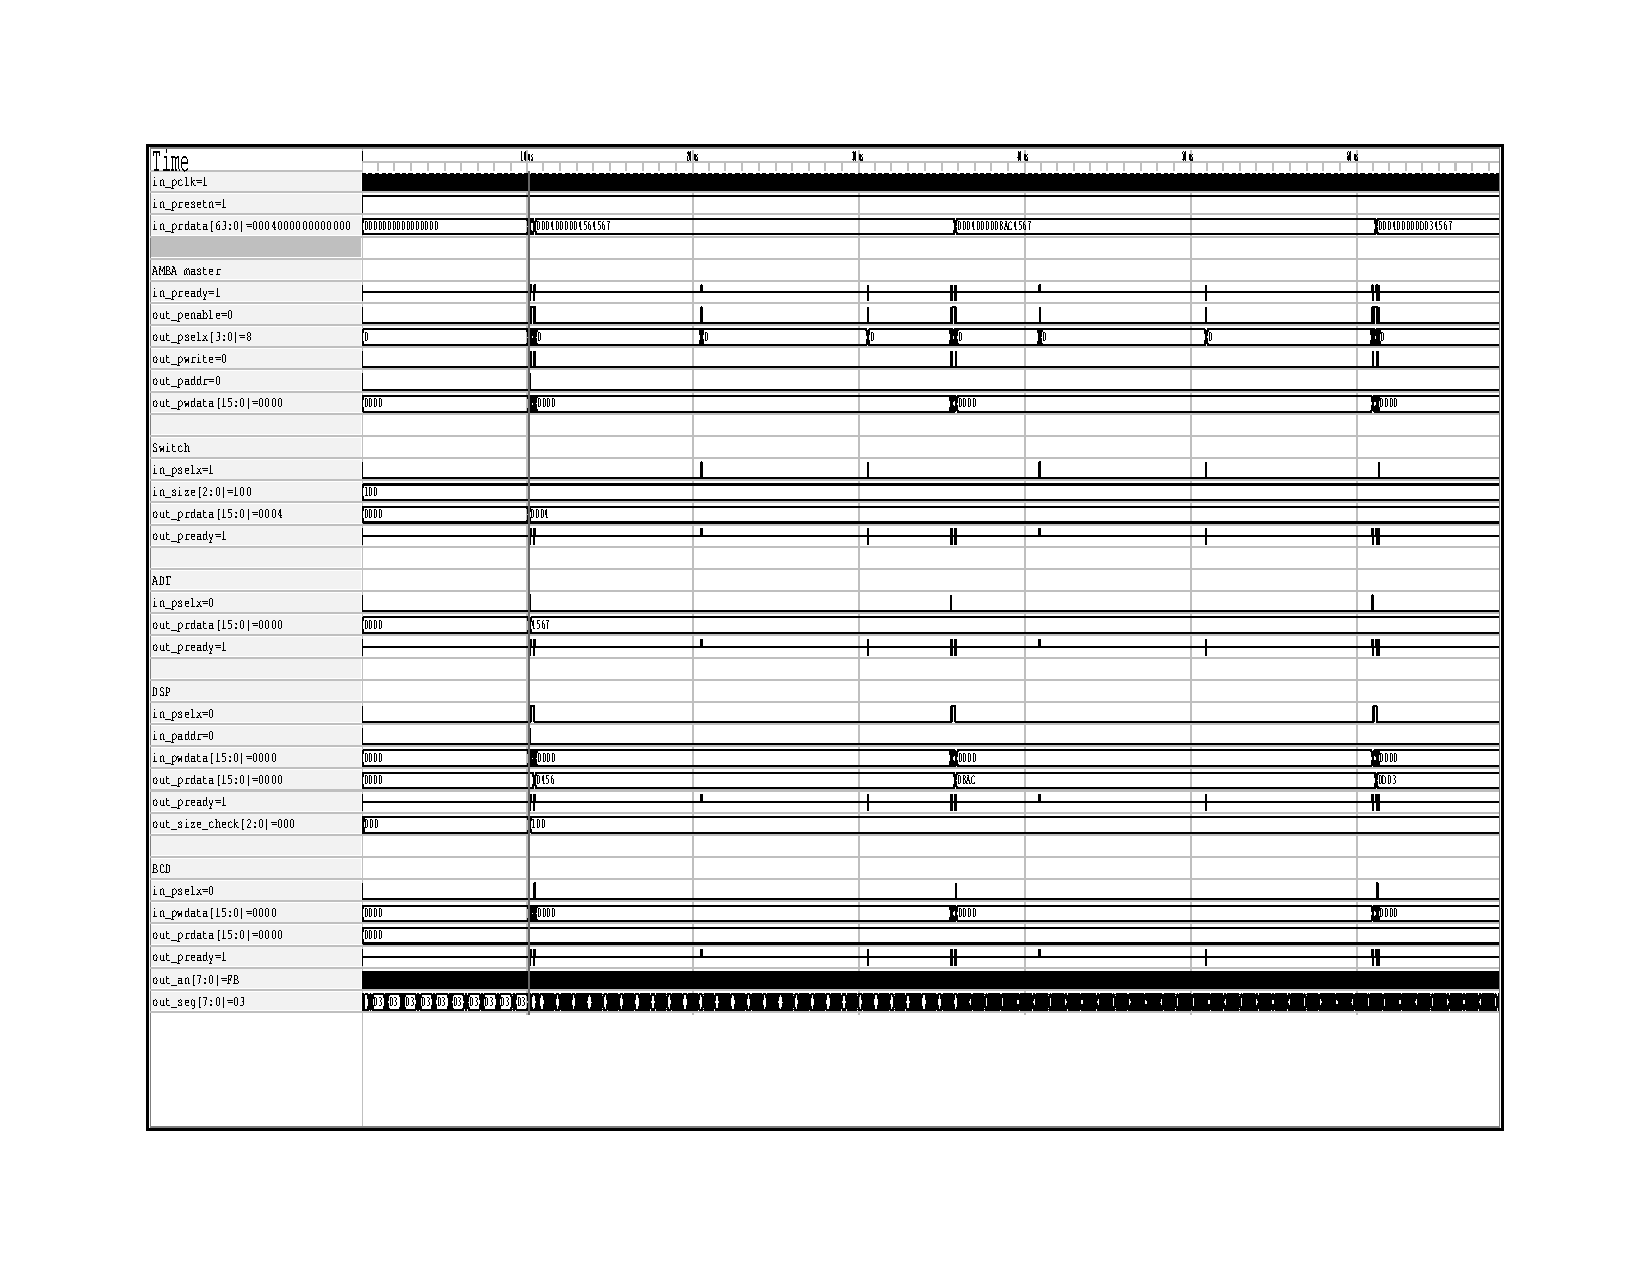
\includepdf[landscape=true,pages=1]{./fig/simulation1.pdf}

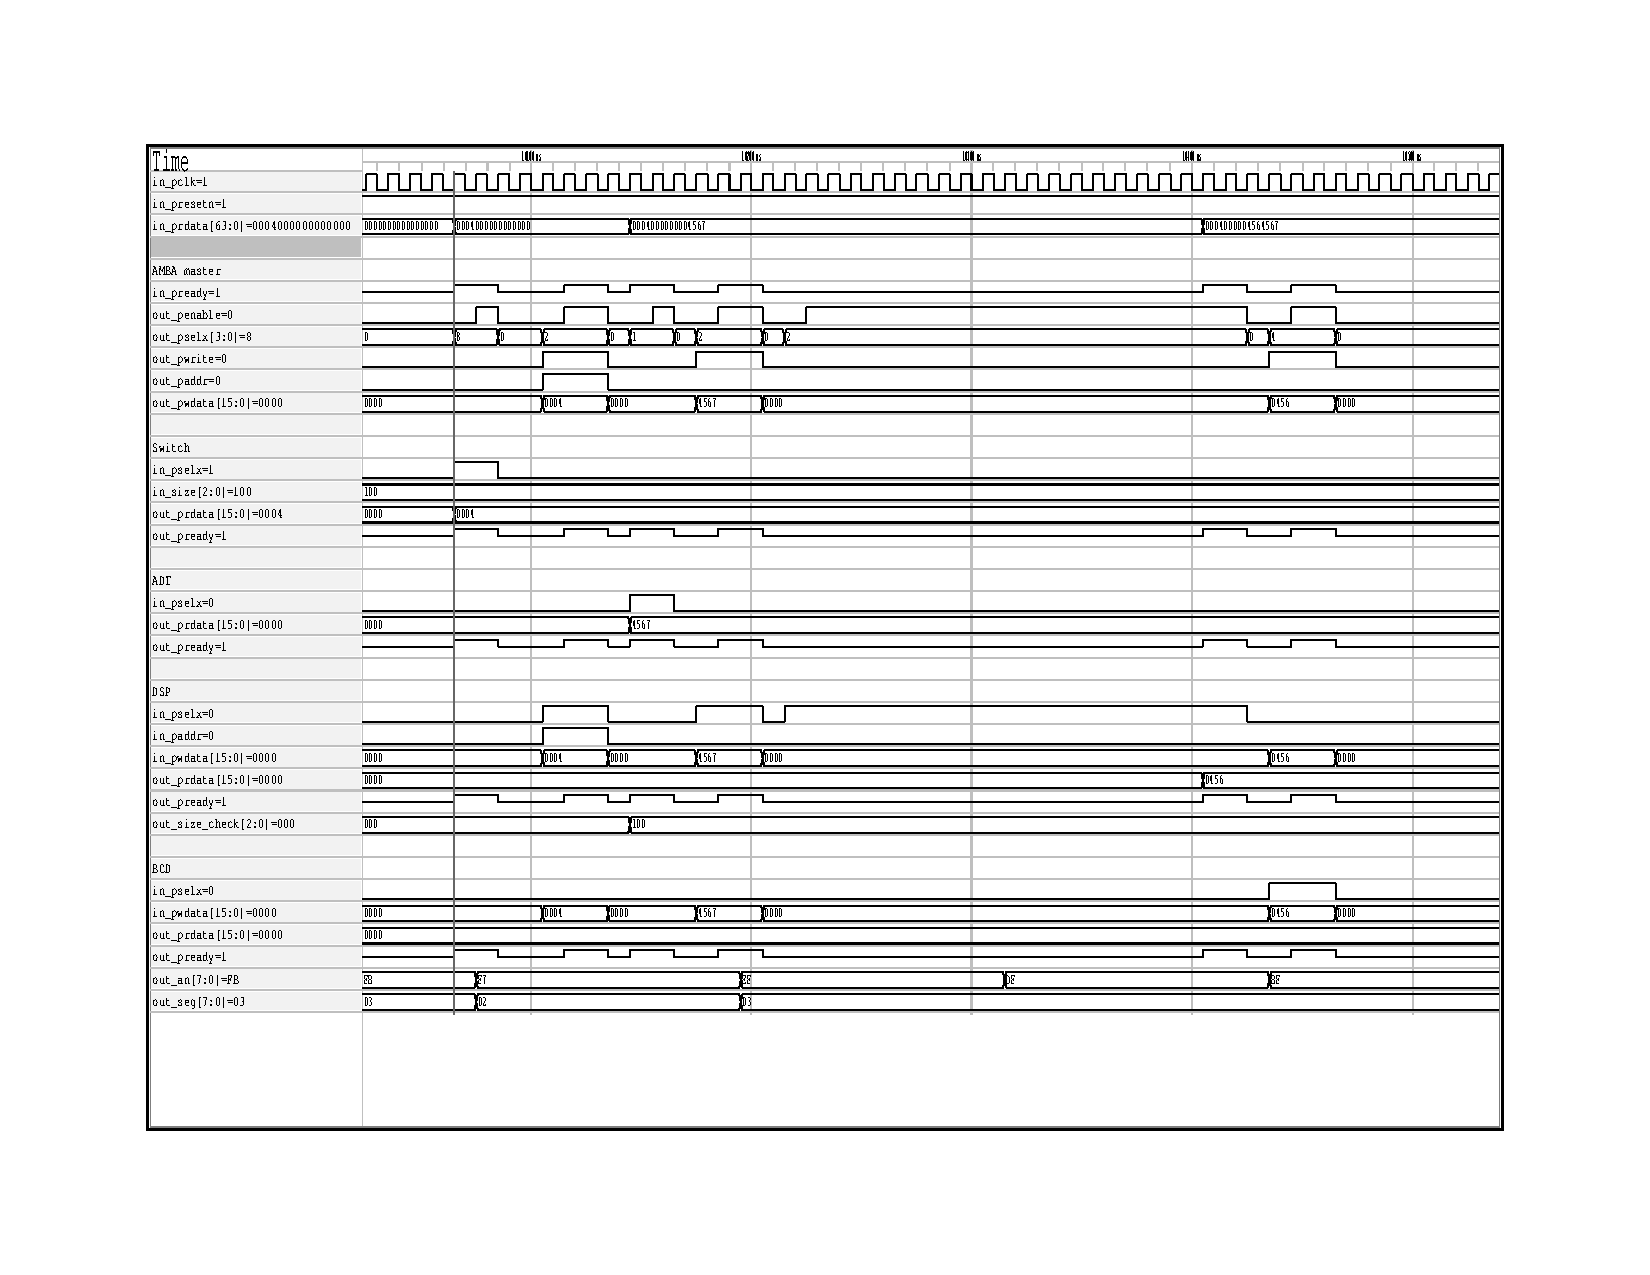
\includepdf[landscape=true,pages=1]{./fig/simulation2.pdf}
\newpage
\subsection{Problems}
I had many problems with my first implementation because I misunderstood a 
central point in the AMBA APB specification. Thanks to this mistake I had
race conditions in my design which caused my simulation to work but my 
implementation to only work sometimes. Much time was wasted by trying it
this way. To clarify my mistake: I tried not to write into registers but
to directly write into the components. By doing it this way I got many
additional conditions to wait for values and multiple sources for enable
signals. Somewhere in between then I got the race condition.

\subsection{Reports}
\subsubsection{utilization report}
\lstinputlisting[basicstyle=\tiny,firstnumber=1]{post_route_utilization.rpt}
\subsubsection{timing report}
In the timing report you can see many pins which are not driven by a clock pin.
This is per design, because APB can react asynchronously to operations. Waiting
for the rising clock edge everytime would always add a wait state.
\lstinputlisting[basicstyle=\tiny,firstnumber=1]{post_route_timing_summary.rpt}

\end{document}
%
%----------------------------------------------------------------------------

